\subsubsection{Simplified Clock and Channel Model Building Blocks for SAL}
\label{ssec:simple_clock_channel}

\lee{Vatsan/Bren/Ben: is this section still relevant for the Sally backend and our current models?}

\ben{I think this section really only applies to how WBS was encoded in SAL.
    The encoding in the ADSL doesn't assume push-push or push-pull, nor does
    it have any notion of node / task clocks.}

While the \emph{push-push} for \emph{synchronous} clock paradigm and \emph{push-pull} for \emph{asynchronous} clock paradigm across a distributed system  described in section \ref{ssec:clock} and channel models described in section \ref{ssec:channel} accurately describes the modeling needs within any ADSL to prove system correctness, it becomes  extremely tricky to implement them within the model-checker as it limited by the ability to express them exactly in the underlying language (e.g. synchronous and asynchronous composition within SAL). Further our end goal is to also model within ADSL (in Phase III) transition of systems from synchronous to asynchronous or vice-versa whereby we can then prove correctness of startup protocol or  synchronization protocol that ensure a common synchronous clock domains can be created and maintained from asynchronous nodes or alternatively system is in safe sate when synchronous domains lose synchronization and breaks down in asynchronous clusters. Towards this end we have made some simplifying requirements we describe in this section, which we then show can be easily implemented in SAL as demonstrated by the case studies described later in section \ref{sec:case-studies}.

\begin{figure}
\begin{center}
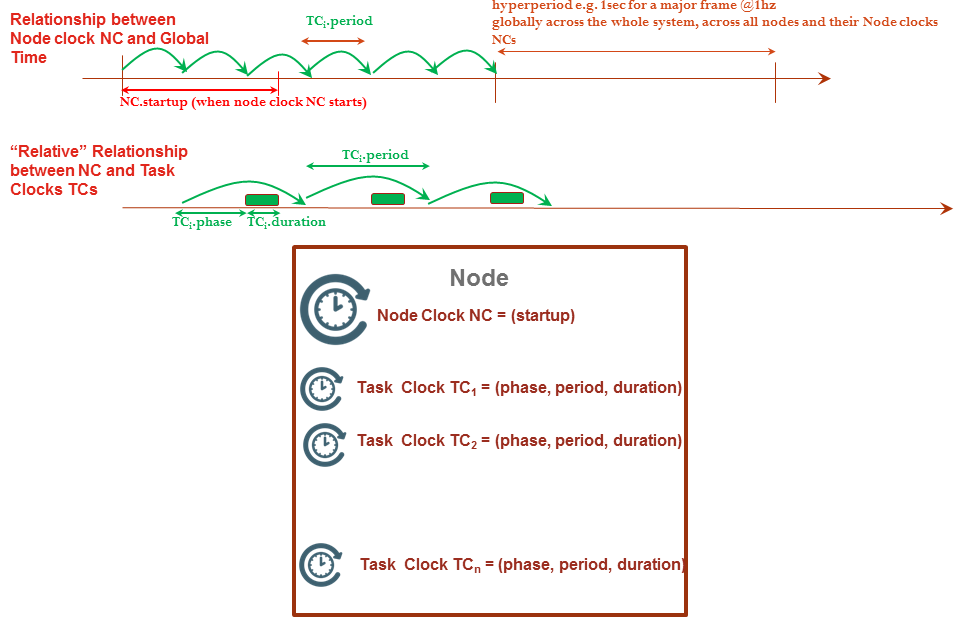
\includegraphics[width=0.8\textwidth]{figures/clocks_overall_node}
\caption{Simplified Node and Task Clock Models}
\label{fig:clocks_overall_node}
\end{center}
\end{figure}

Every node in a distributed system then is modeled with a single \emph{Node Clock} and a bunch of associated \emph{Task Clocks} along with it. This is illustrated in figure \ref{fig:clocks_overall_node}. Every Node’s Clock (NC) exclusively drives all Task Clocks (TCs) within the node.  The NC within a node is defined by the variable $NC=(startup)$ that described the relationship between the Node's clock and an ideal global notion of time across all nodes. More precisely it specifies when the node's clock starts ticking with respect to this global time and can be specified as a "startup" phase offset within a hyper-period. Hyperperiod is a major frame of all associated tasks i.e. \emph{Least Common Multiple (LCM)} of periods of all TCs modeled within the system across all nodes. Thus for the rest of our discussion all TC periods are harmonic with respect to this hyperperiod. The temporal dependencies between NC and TCs can be captured as constraints, $\forall i \leq n$:
\begin{itemize}
\item $\exists k \in \mathbb{Z}^+, k \times TC_i.period = 1 sec$. Example when $TC_i$ periods are harmonic to $hyperperiod = 1 sec$. In the model $TC_i.period$ are model \emph{constants} pre-defined apriori and static (unvarying)
\item $0 \leq NC.startup \leq 1 sec$. In the model $TC_i.startup$ are model \emph{variables} which the model checker will vary and explore
\end{itemize}

\begin{figure}
\begin{center}
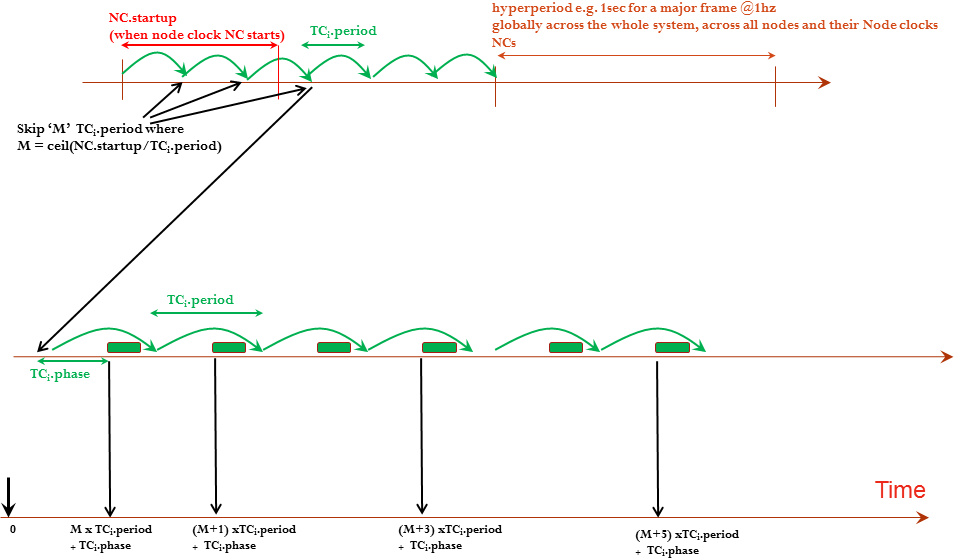
\includegraphics[width=0.8\textwidth]{figures/node_task_clocks}
\caption{Progression of Time based on NC and TCs}
\label{fig:node_task_clocks}
\end{center}
\end{figure}

NC and TCs are expected to be asynchronously composed with each other within SAL. NCs are then described by the parameters $TC_i = (phase,period, duration)$ and these are "relative" with respect to the $NC=(startup)$ within the node and individually denotes the phase within period, period and duration of tasks respectively as shown in figure \ref{fig:clocks_overall_node}. The expectation is that if any task (computation or communication) modeled within a node is driven by a task clock $TC$, then $duration$ represents the CPU time in case of computation task (e.g. execution time of program or logic) or alternatively in the case of communication task represents appropriate channel transmission or reception (plus processing overhead) delays encountered during communication over a channel or network. The TC constraints can be captured as, $\forall i \leq n$:
\begin{itemize}
\item $0 \leq TC_i.period$ where $TC_i.period$ are model \emph{constants} pre-defined apriori and static (unvarying)
\item $0 \leq TC_i.phase$ where $TC_i.phase$ are  model \emph{variables} to be varied and explored by model checker
\item $0 \leq TC_i.duration$ where $TC_i.duration$ are model \emph{constants} pre-defined apriori and static (unvarying)
\item $0 \leq TC_i.phase + TC_i.duration \leq TC_i.period$
\end{itemize}

The progression of time and resultant time of TC function of $NC.startup$ and $TC_i.phase$ is shown in figure \ref{fig:node_task_clocks}. $NC.startup$  and $TC_i.phase$ together determines periodic “starting” times of tasks associated with TC clocks. Essentially the task clocks are \emph{temporally shifted right} by additional $M \times TC_i.period$s initially to account of the node clocks startup $NC.startup$ where $M=\lceil\frac{NC.startup}{TC_i.period}\rceil$. Further additional temporal dependencies, if any, between tasks as shown in figure \ref{fig:task_clock_dependencies}, can also be easily modeled and captured as constraints.  For example, for some tasks $i$ and $j$, if we want to satisfy the temporal dependency that $TC_i$ always occurs before $TC_j$, then specify the constraint in the model as $i,j \leq n$:
\begin{itemize}
\item $TC_i.period = TC_j.period$. Only works when the two clocks are the same periods
\item $0 \leq TC_i.phase + TC_i.duration \leq TC_j.phase$
\end{itemize}

\begin{figure}
\begin{center}
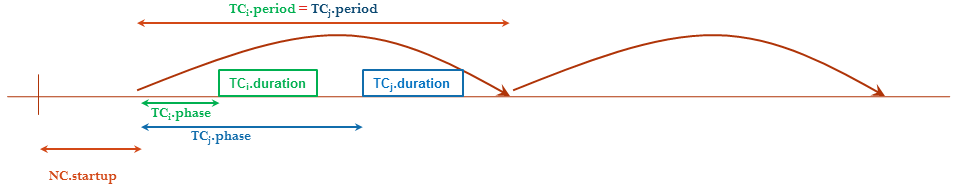
\includegraphics[width=0.8\textwidth]{figures/task_clock_dependencies}
\caption{Additional Temporal Task Dependencies}
\label{fig:task_clock_dependencies}
\end{center}
\end{figure}

Consider two nodes $Node_1$ and $Node_2$ with their node clocks $Node_1.NC=(startup)$ and  $Node_2.NC=(startup)$. If the two nodes are \emph{asynchronous} with each other i.e. their corresponding node clocks are asynchronous, then the model checker simply explores $NC.startup$ completely  using the constraint $-\Omega \leq (Node_1.NC.startup - Node_2.NC.startup) \leq +\Omega$ where $\Omega = LCM(TC_i.period), \forall TC_i \in Node_1 \bigcup Node_2 $. $LCM$ is the least common multiple.

Alternatively, If the two nodes are \emph{synchronous} with each other i.e. their corresponding node clocks are synchronous, then the model checker simply explores $NC.startup$ completely  using the constraint $-\Delta \leq (Node_1.NC.startup - Node_2.NC.startup) \leq +\Delta$ where $\Delta \ll GCD(TC_i.period), \forall TC_i \in Node_1 \bigcup Node_2 $. $GCD$ is the greatest common divisor. Essentially explore $NC.startup$ within a very small system \emph{synchronization precision constant} $\Delta$. For such \emph{synchronous} clocks, add additional constraints to the model $\forall TC_i \in Node_1 \bigcup Node_2: \langle 0 \leq TC_i.phase \leq 2\Delta\rangle$. Hence upper bounds $TCi.phase$ is subsequently limited to be explored in terms of the "smaller" $\Delta$ achieved due to synchronization and hence the smaller deviation between their corresponding node clocks $NC.startup$. 

\begin{figure}
\begin{center}
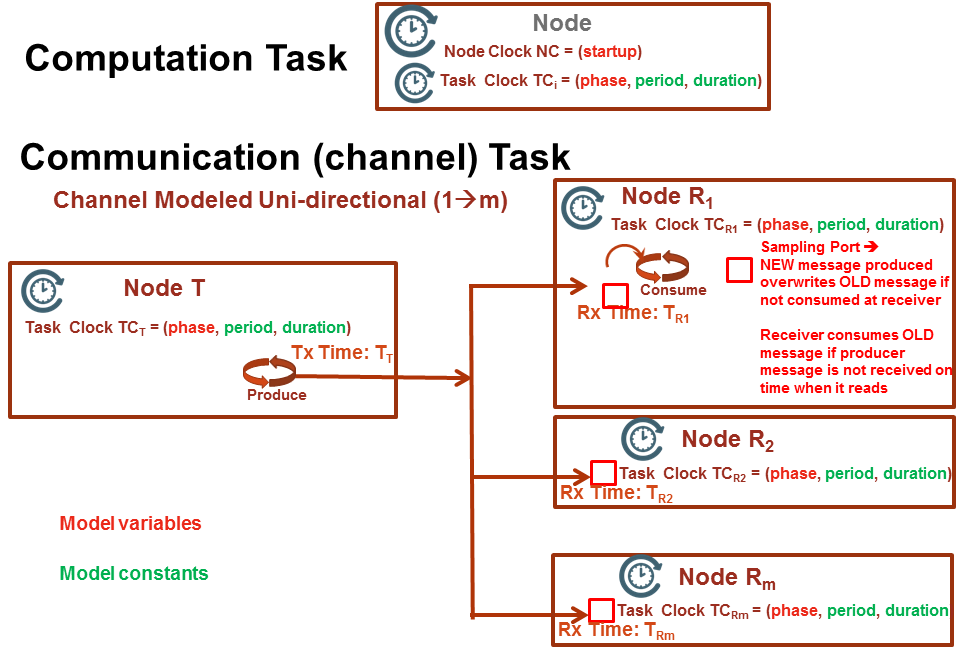
\includegraphics[width=0.8\textwidth]{figures/compute_comm_model}
\caption{Computation and Communication (Channel) models}
\label{fig:compute_comm_model}
\end{center}
\end{figure}

In figure \ref{fig:compute_comm_model} we show how the computation and communication via a channel can then be modeled using the clocks paradigm described above. $duration$ and $period$ are just model constants in computation task with clock $TC_i$ indicates the periodicity of the task and the execution time of the task within each period. Observe that both $duration$ and $period$ are model constants in which the model checker does not “explore”. Only model variables $phase$ in $TC_i$ and $startup$ in node clock $NC$ are explored by model checker. Notice that feasible task schedule exists if $\forall Node_k: \langle \sum_{\forall TC_i \in Node_k} \frac{TC_i.duration}{TC_i.period} \leq 1.0 \rangle$. Hence the feasibility of task schedule and an actual task schedule is not determined by model checking. It is determined all statically upfront by specifying them properly as constants into the models.

The communication task shown in figure \ref{fig:compute_comm_model} involves a channel modeled uni-directional $1 \rightarrow m$ from transmitter node $T$ with task clock $TC_T$ to node receivers $R_1,R_2,...,R_m$ and corresponding tasks clocks $TC_{R_1},TC_{R_2},...,TC_{R_m}$. $duration$ on $TC_T$ indicates the message produce latency i.e. time to create a message while $duration$ on $TC_{R_i}$ indicates the network/channel delay for message to be transmitted from Node $T$, propagate through the network all the way till it is consumed at receiver $R_i$. As before note that $phase$ for task clocks $TC$ are model variables while $duration$ and $period$ of task clocks $TC$ are model constants. The sampling port at the receiver for communication channel buffer model described in section \ref{ssec:channel} is a feature whereby new message produced by the transmitter overwrites old message if not consumed at receiver and also receiver consumes old message if produce message from the transmitter  is not received on time when the receiver reads the port.  This sampling port feature can be specified as constraints on transmission time (Tx) Time $T_T$ and receptions times (Rx) $T_{R_i}$ as:
\begin{equation*}\forall i, 1 \leq i \leq m: \left< \begin{array}{l} \text{If } T_{R_i} \geq T_T + TC_T.duration + TC_{R_i}.duration \Longrightarrow \text{New Message} \\ \text{Else } \Longrightarrow \text{Old Message} \end{array} \right> \end{equation*}

Thus as shown above \emph{Asynchronous and Synchronous clock paradigm are easily specified as additional constraints within the model}. Furthermore \emph{there is a simple way to express both type of Computation and Communication tasks}.




